\section{特征方程}
\label{sec:hj-characteristics}

方程只说了时间导数和梯度的关系，能否沿某些曲线把它化成常微分方程？输运方程已经用过这个办法：沿速度场的轨线，解的值不变。这里的困难在于，方程对梯度非线性，沿曲线求导时会冒出二阶导数。这一节要找到让二阶导数消失的曲线，并说明怎样从这些曲线重建场。

\paragraph{沿什么曲线求导}
设$H$二阶连续可微，$u$是二阶连续可微的经典解。取一条待定的曲线$\bm{x}(s)$，记沿线的梯度和值为
\[
  \bm{p}(s)=\nabla u(\bm{x}(s),s),\qquad z(s)=u(\bm{x}(s),s).
\]
对$\bm{p}$求导，用链式法则，得到
\[
  \dot{\bm{p}}=\partial_t\nabla u+\nabla^2u\,\dot{\bm{x}}.
\]
这里出现了未知的二阶导数$\nabla^2u$，这是方程非线性的代价。

为消去$\partial_t\nabla u$，对方程本身关于$\bm{x}$求梯度：
\[
  \partial_t\nabla u+\nabla_{\bm{x}}H+\nabla^2u\,\nabla_{\bm{p}}H=0.
\]
两式相减消去$\partial_t\nabla u$，得到
\[
  \dot{\bm{p}}=-\nabla_{\bm{x}}H+\nabla^2u\,\bigl(\dot{\bm{x}}-\nabla_{\bm{p}}H\bigr).
\]
括号里的量可以由我们选择：只要曲线满足$\dot{\bm{x}}=\nabla_{\bm{p}}H$，二阶导数就消失了。曲线的方向不是事先给定的速度场，而由当地的斜率决定。

再算沿线的值。由链式法则和方程，
\[
  \dot{z}=\partial_tu+\langle\nabla u,\dot{\bm{x}}\rangle=-H+\langle\bm{p},\nabla_{\bm{p}}H\rangle.
\]
把这三个结果写在一起。

\begin{theorem}[特征方程组]
\label{thm:hj-characteristics}
设$H\in C^2$，$u\in C^2$是方程$\partial_tu+H(t,\bm{x},\nabla u)=0$的解。若曲线$\bm{x}(s)$的速度等于$\nabla_{\bm{p}}H$（梯度变量取沿线的$\nabla u$），则沿线的梯度$\bm{p}(s)$和值$z(s)$满足
\begin{equation}
  \dot{\bm{x}}=\nabla_{\bm{p}}H,\qquad
  \dot{\bm{p}}=-\nabla_{\bm{x}}H,\qquad
  \dot{z}=\langle\bm{p},\nabla_{\bm{p}}H\rangle-H,
  \label{eq:hj-characteristics}
\end{equation}
其中$H$及其偏导数都在$(s,\bm{x}(s),\bm{p}(s))$处取值。这组常微分方程称为\term{特征方程组}（characteristic system），$\bm{x}(s)$称为特征线。
\end{theorem}

式~\eqref{eq:hj-characteristics}的前两个方程不含$z$，构成$(\bm{x},\bm{p})$空间中的闭合系统，这就是第~\ref{chap:ode-sensitivity}章的Hamilton方程。在那里我们已经知道它生成的流保持相空间体积，$H$不显含时间时沿轨道守恒。这两条性质这里不再重复；本章的新内容是第三个方程，它在已知$(\bm{x},\bm{p})$之后只是一次积分，负责把值带上。

图~\ref{fig:hj-characteristic-lift}是一条特征线的示意。出发点$\bm{y}$提供初始斜率$\bm{p}_0=\nabla u_0(\bm{y})$，此后位置按$\nabla_{\bm{p}}H$前进，斜率按$-\nabla_{\bm{x}}H$变化，值按第三式累积。

\begin{BookInlineFigure}
  \centering
  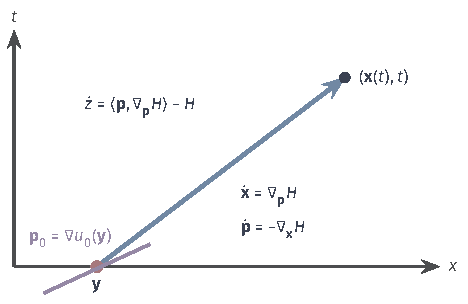
\includegraphics[width=79.3mm]{figures/06-differential-equations/02-partial-differential-equations/tikz/hj-characteristic-lift/figure.pdf}
  \caption{一条特征线（蓝）。从初始点$\bm{y}$（红）出发，紫线表示初值在该点的切线，它给出初始斜率$\bm{p}_0$。沿线要同时求解位置、斜率和值三个量。}
  \label{fig:hj-characteristic-lift}
\end{BookInlineFigure}

\paragraph{由特征重建场}
定理~\ref{thm:hj-characteristics}假定解已经存在，只是必要条件。反过来，给定$u_0$，能否从特征线造出解？做法分三步。

\begin{enumerate}
  \item 对每个$\bm{y}$，从位置$\bm{y}$、斜率$\nabla u_0(\bm{y})$、值$u_0(\bm{y})$出发解式~\eqref{eq:hj-characteristics}，得到$\bm{x}(\bm{y},t)$、$\bm{p}(\bm{y},t)$、$z(\bm{y},t)$。
  \item 对给定的$(\bm{x},t)$，解方程$\bm{x}(\bm{y},t)=\bm{x}$，求出是哪条特征线到达这里。
  \item 令$u(\bm{x},t)=z(\bm{y},t)$，其中$\bm{y}$是上一步的解。
\end{enumerate}

第二步是关键：只有映射$\bm{y}\mapsto\bm{x}(\bm{y},t)$可逆时，$u$才有定义。$t=0$时它是恒等映射，所以短时间内可逆，这用到反函数定理：Jacobian可逆的连续可微映射局部有连续可微的逆，可参考\BookChapterRef{chap:implicit-inverse-functions}{卷二第22章“隐函数与反函数”}。这一步还需要证明造出来的函数确实满足方程，而不只是沿线有正确的取值。

\begin{theorem}[经典解的局部存在]
\label{thm:hj-local-classical}
设$H\in C^2$，$u_0\in C^2$。对每个$\bm{y}_0\in\mathbb{R}^{d}$，存在$t_1>0$和$\bm{y}_0$的邻域，使上面三步在$\bm{x}(\bm{y}_0,t)$附近、$0\leq t<t_1$时定义出一个连续可微函数$u$，它满足
\begin{equation}
  \partial_tu+H(t,\bm{x},\nabla u)=0,\qquad u(\cdot,0)=u_0,\qquad\nabla u(\bm{x}(\bm{y},t),t)=\bm{p}(\bm{y},t).
  \label{eq:hj-local-classical}
\end{equation}
\end{theorem}

\begin{proof}
式~\eqref{eq:hj-characteristics}的右端关于$(\bm{x},\bm{p})$连续可微，初值关于$\bm{y}$连续可微，所以解关于$\bm{y}$连续可微。映射$(\bm{y},t)\mapsto(\bm{x}(\bm{y},t),t)$在$t=0$处的Jacobian是单位阵，由反函数定理局部可逆，$u$有定义且连续可微。

关键是证明$\nabla u=\bm{p}$。固定指标$i$，记$\partial_i=\partial/\partial y_i$，考虑
\[
  a(t)=\partial_iz-\langle\bm{p},\partial_i\bm{x}\rangle.
\]
$t=0$时，$\partial_iz=\partial_iu_0(\bm{y})$，$\partial_i\bm{x}=\bm{e}_i$，$\bm{p}=\nabla u_0(\bm{y})$，所以$a(0)=0$。

下面计算$\dot{a}$。对$\dot{z}=\langle\bm{p},\nabla_{\bm{p}}H\rangle-H$关于$y_i$求导，其中含$\partial_i\bm{p}$的两项抵消：
\[
  \partial_i\dot{z}=\langle\bm{p},\partial_i(\nabla_{\bm{p}}H)\rangle-\langle\nabla_{\bm{x}}H,\partial_i\bm{x}\rangle.
\]
另一方面，由$\dot{\bm{p}}=-\nabla_{\bm{x}}H$和$\dot{\bm{x}}=\nabla_{\bm{p}}H$，
\[
  \frac{\mathrm{d}}{\mathrm{d}t}\langle\bm{p},\partial_i\bm{x}\rangle=-\langle\nabla_{\bm{x}}H,\partial_i\bm{x}\rangle+\langle\bm{p},\partial_i(\nabla_{\bm{p}}H)\rangle.
\]
两式相减，$\dot{a}=0$，于是$a\equiv0$，即对所有$i$有$\partial_iz=\langle\bm{p},\partial_i\bm{x}\rangle$。

由$u$的定义和链式法则，又有
\[
  \partial_iz=\langle\nabla u,\partial_i\bm{x}\rangle.
\]
比较两式，得
\[
  \langle\nabla u-\bm{p},\partial_i\bm{x}\rangle=0,\qquad i=1,\ldots,d.
\]
向量$\partial_1\bm{x},\ldots,\partial_d\bm{x}$线性无关，所以$\nabla u=\bm{p}$。

最后对$z(\bm{y},t)=u(\bm{x}(\bm{y},t),t)$关于$t$求导，并代入$\dot{z}$的方程和$\nabla u=\bm{p}$：
\[
  \langle\bm{p},\nabla_{\bm{p}}H\rangle-H=\partial_tu+\langle\bm{p},\nabla_{\bm{p}}H\rangle.
\]
消去相同的项，得到$\partial_tu=-H$。
\end{proof}

下面用一个可以手算的例子走一遍这三步。这个例子会贯穿到最后一节。

\begin{example}[余弦初值]
\label{ex:hj-cos}
取$d=1$，$H(p)=p^2/2$，$u_0(x)=\cos x$。特征方程组是
\[
  \dot{x}=p,\qquad\dot{p}=0,\qquad\dot{z}=\frac{p^2}{2}.
\]
从$y$出发，初始斜率$p=-\sin y$沿线不变，特征线是直线，于是
\[
  x=y-t\sin y,\qquad p=-\sin y,\qquad z=\cos y+\frac{t}{2}\sin^2y.
\]

取$t=1/2$、$y=\pi/2$，得到
\[
  x=\frac{\pi}{2}-\frac12,\qquad p=-1,\qquad z=\frac14.
\]
因此$u(\pi/2-1/2,\ 1/2)=1/4$，该点的斜率是$-1$。$t=1/2$时$\partial x/\partial y=1-\frac12\cos y>0$，$y\mapsto x$严格单调，这个点只由这一条特征线到达。
\end{example}

\paragraph{到达时间的特征线}
对波前对应的$H(\bm{x},\bm{p})=c(\bm{x})\lVert\bm{p}\rVert_2$（$\bm{p}\neq\bm{0}$），偏导数是
\[
  \nabla_{\bm{p}}H=c\,\frac{\bm{p}}{\lVert\bm{p}\rVert_2},\qquad\nabla_{\bm{x}}H=\lVert\bm{p}\rVert_2\nabla c.
\]
代入式~\eqref{eq:hj-characteristics}，第一个方程说特征线沿$\bm{p}$的方向以速度$c$前进，这条曲线叫射线。第三个方程给出
\[
  \dot{z}=\Bigl\langle\bm{p},c\frac{\bm{p}}{\lVert\bm{p}\rVert_2}\Bigr\rangle-c\lVert\bm{p}\rVert_2=0.
\]
也就是说，$u=T-t$沿射线不变，这正是波前的含义：射线上的点时刻$s$恰好在波前上，$T(\bm{x}(s))$每经过单位时间增加$1$。

图~\ref{fig:hj-huygens}从另一个角度解释射线。把当前波前上的每个点当作新的小波源，小圆的公共包络就是下一时刻的波前，连接圆心和切点的方向就是射线方向。这就是几何上的波前图景，也说明射线垂直于波前（速度$c$只依赖位置时）。

\begin{BookInlineFigure}
  \centering
  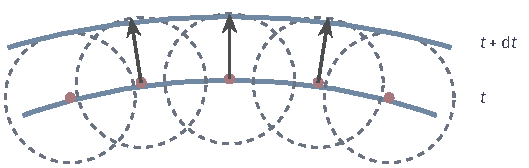
\includegraphics[width=89.5mm]{figures/06-differential-equations/02-partial-differential-equations/tikz/hj-huygens/figure.pdf}
  \caption{波前的包络图景。下方蓝线是时刻$t$的波前，红点发出半径$c\,\mathrm{d}t$的小圆（虚线），上方蓝线是这些小圆的包络，即$t+\mathrm{d}t$的波前，深灰箭头是射线。}
  \label{fig:hj-huygens}
\end{BookInlineFigure}

速度为常数时，$\nabla c=\bm{0}$，$\bm{p}$不变，射线是直线，$T$就是到源点的距离除以$c$。速度随位置变化时射线弯曲。例如在平面上取$c(\bm{x})=1+ax_2$，$a=1/2$，源在原点。这个速度下到达时间有闭式
\begin{equation}
  T(\bm{x})=\frac{1}{a}\operatorname{arccosh}\Bigl(1+\frac{a^2\lVert\bm{x}\rVert_2^2}{2c(\bm{x})}\Bigr),
  \label{eq:hj-linear-speed}
\end{equation}
代入程函方程可以验证。我们沿竖直射线手算一个点：在$x_1=0$上向上走，$\dot{x}_2=1+x_2/2$，$x_2(0)=0$，解得
\[
  x_2(t)=2\bigl(\mathrm{e}^{t/2}-1\bigr).
\]
令$x_2=2$，得到$t=2\ln2\approx1.386$。式~\eqref{eq:hj-linear-speed}在$(0,2)$处给出$\operatorname{arccosh}(1.25)/a=2\ln2$，两者一致。

图~\ref{fig:hj-rays-linear-speed}用数值积分解特征方程组，得到射线，再画上式~\eqref{eq:hj-linear-speed}的等值线。射线总向速度小的一侧弯转，斜向上出发的射线进入快层后又折回下方。射线与等值线处处垂直。积分到$t=3.2$时，射线终点的$T$值与$t$的差不超过$2\times10^{-11}$。

\begin{BookInlineFigure}
  \centering
  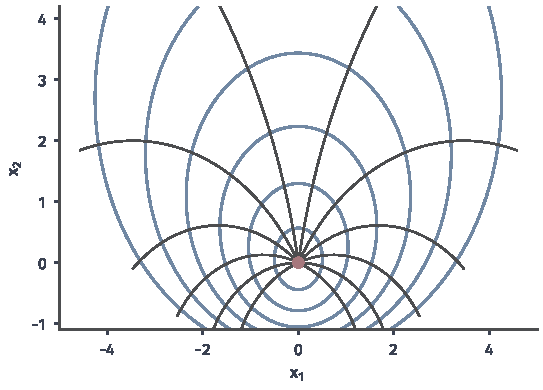
\includegraphics[width=92mm]{figures/06-differential-equations/02-partial-differential-equations/matplotlib/hj-rays-linear-speed/figure.pdf}
  \caption{速度$c=1+x_2/2$下从原点（红）出发的波前和射线。蓝线是式~\eqref{eq:hj-linear-speed}在$T=0.5,1,\ldots,3$的等值线，深灰线是用步长$0.01$的四阶Runge--Kutta方法积分特征方程组得到的射线，初始方向间隔$20^\circ$。}
  \label{fig:hj-rays-linear-speed}
\end{BookInlineFigure}

\paragraph{边界数据怎样启动特征线}
初值问题的特征线从每个$\bm{y}$以确定的斜率出发。程函方程的数据只在$\Gamma$上给出值，切向导数能由$g$算出，法向导数却要由方程决定。设$\Gamma$是一段超曲面，$\nabla_\Gamma g$是$g$沿$\Gamma$的切向梯度，$\bm{n}$是单位法向。令$\bm{p}=\nabla_\Gamma g+\beta\bm{n}$，代入$\lVert\bm{p}\rVert_2=1/c$，得到
\begin{equation}
  \beta=\pm\sqrt{\frac{1}{c^2}-\lVert\nabla_\Gamma g\rVert_2^2}.
  \label{eq:hj-boundary-branches}
\end{equation}
图~\ref{fig:hj-boundary-branches}的圆是$\lVert\bm{p}\rVert_2=1/c$，竖直虚线是切向分量固定时的所有候选，两个交点就是式~\eqref{eq:hj-boundary-branches}的两支。

\begin{BookInlineFigure}
  \centering
  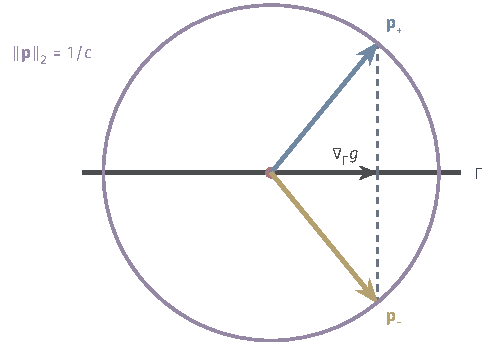
\includegraphics[width=83.5mm]{figures/06-differential-equations/02-partial-differential-equations/tikz/hj-boundary-branches/figure.pdf}
  \caption{边界上的初始斜率。紫圆是$\lVert\bm{p}\rVert_2=1/c$，水平线是边界$\Gamma$，切向分量$\nabla_\Gamma g$由数据给定，方程留下两支法向分量：$\bm{p}_+$（蓝）指向一侧，$\bm{p}_-$（黄）指向另一侧。}
  \label{fig:hj-boundary-branches}
\end{BookInlineFigure}

要使两支是不同的实数，需要$\lVert\nabla_\Gamma g\rVert_2<1/c$。它的含义是：起始时刻沿$\Gamma$变化得不能太快。沿$\Gamma$的视在传播速度$1/\lVert\nabla_\Gamma g\rVert_2$要大于当地的波速$c$。若$g$沿$\Gamma$变化得更快，某个点规定的起始时刻已晚于别的点传来的波前，就是第~\ref{sec:hj-problem}节$g(1)=2$的情形。选定一支后，就得到从$\Gamma$的一侧发出的波前。
